% !TEX root = main.tex
\chapter{Flavour Tagging am \lhcb Experiment}

Um die \CP-Verletzung in der Interferenz aus Mischung und Zerfall zu messen, muss der initiale Flavour des zerfallenden \B-Mesons bekannt sein, also ob es sich um ein \Bz- oder ein \Bzb-Meson handelt (Gleichung \eqref{eq:cpv}). Dies wird bei \lhcb durch das sogenannte Flavour Tagging festgestellt. Dabei geben verschiedene Algorithmen (Tagger) für jeden Kandidaten sowohl eine Entscheidung darüber, um welchen Flavour es sich gehandelt hat, als auch eine Wahrscheinlichkeit mit der Entscheidung falsch zu liegen, aus. Es wird dabei zwischen Taggern der Same Side (SS) und Taggern der Opposite Side (OS) unterschieden. Die SS Tagger untersuchen Teilchen, die in direktem Zusammenhang mit dem Hadronisierungsprozess entstehen, der beim Signal \bquark-Quark abläuft. Die OS Tagger analysieren den Hadronisierungsprozess des zweiten, mit dem Signal \bquark-Quark (\bquarkbar-Quark) gemeinsam erzeugten \bquarkbar-Quarks (\bquark-Quark) (Abbildung \ref{fig:flavourtagging}). Zum Abschluss wird schließlich die Selbsteinschätzung der Tagger zu einer \enquote{wahren} Wahrscheinlichkeit umgerechnet. 
\begin{figure}[htpb]
	\centering
		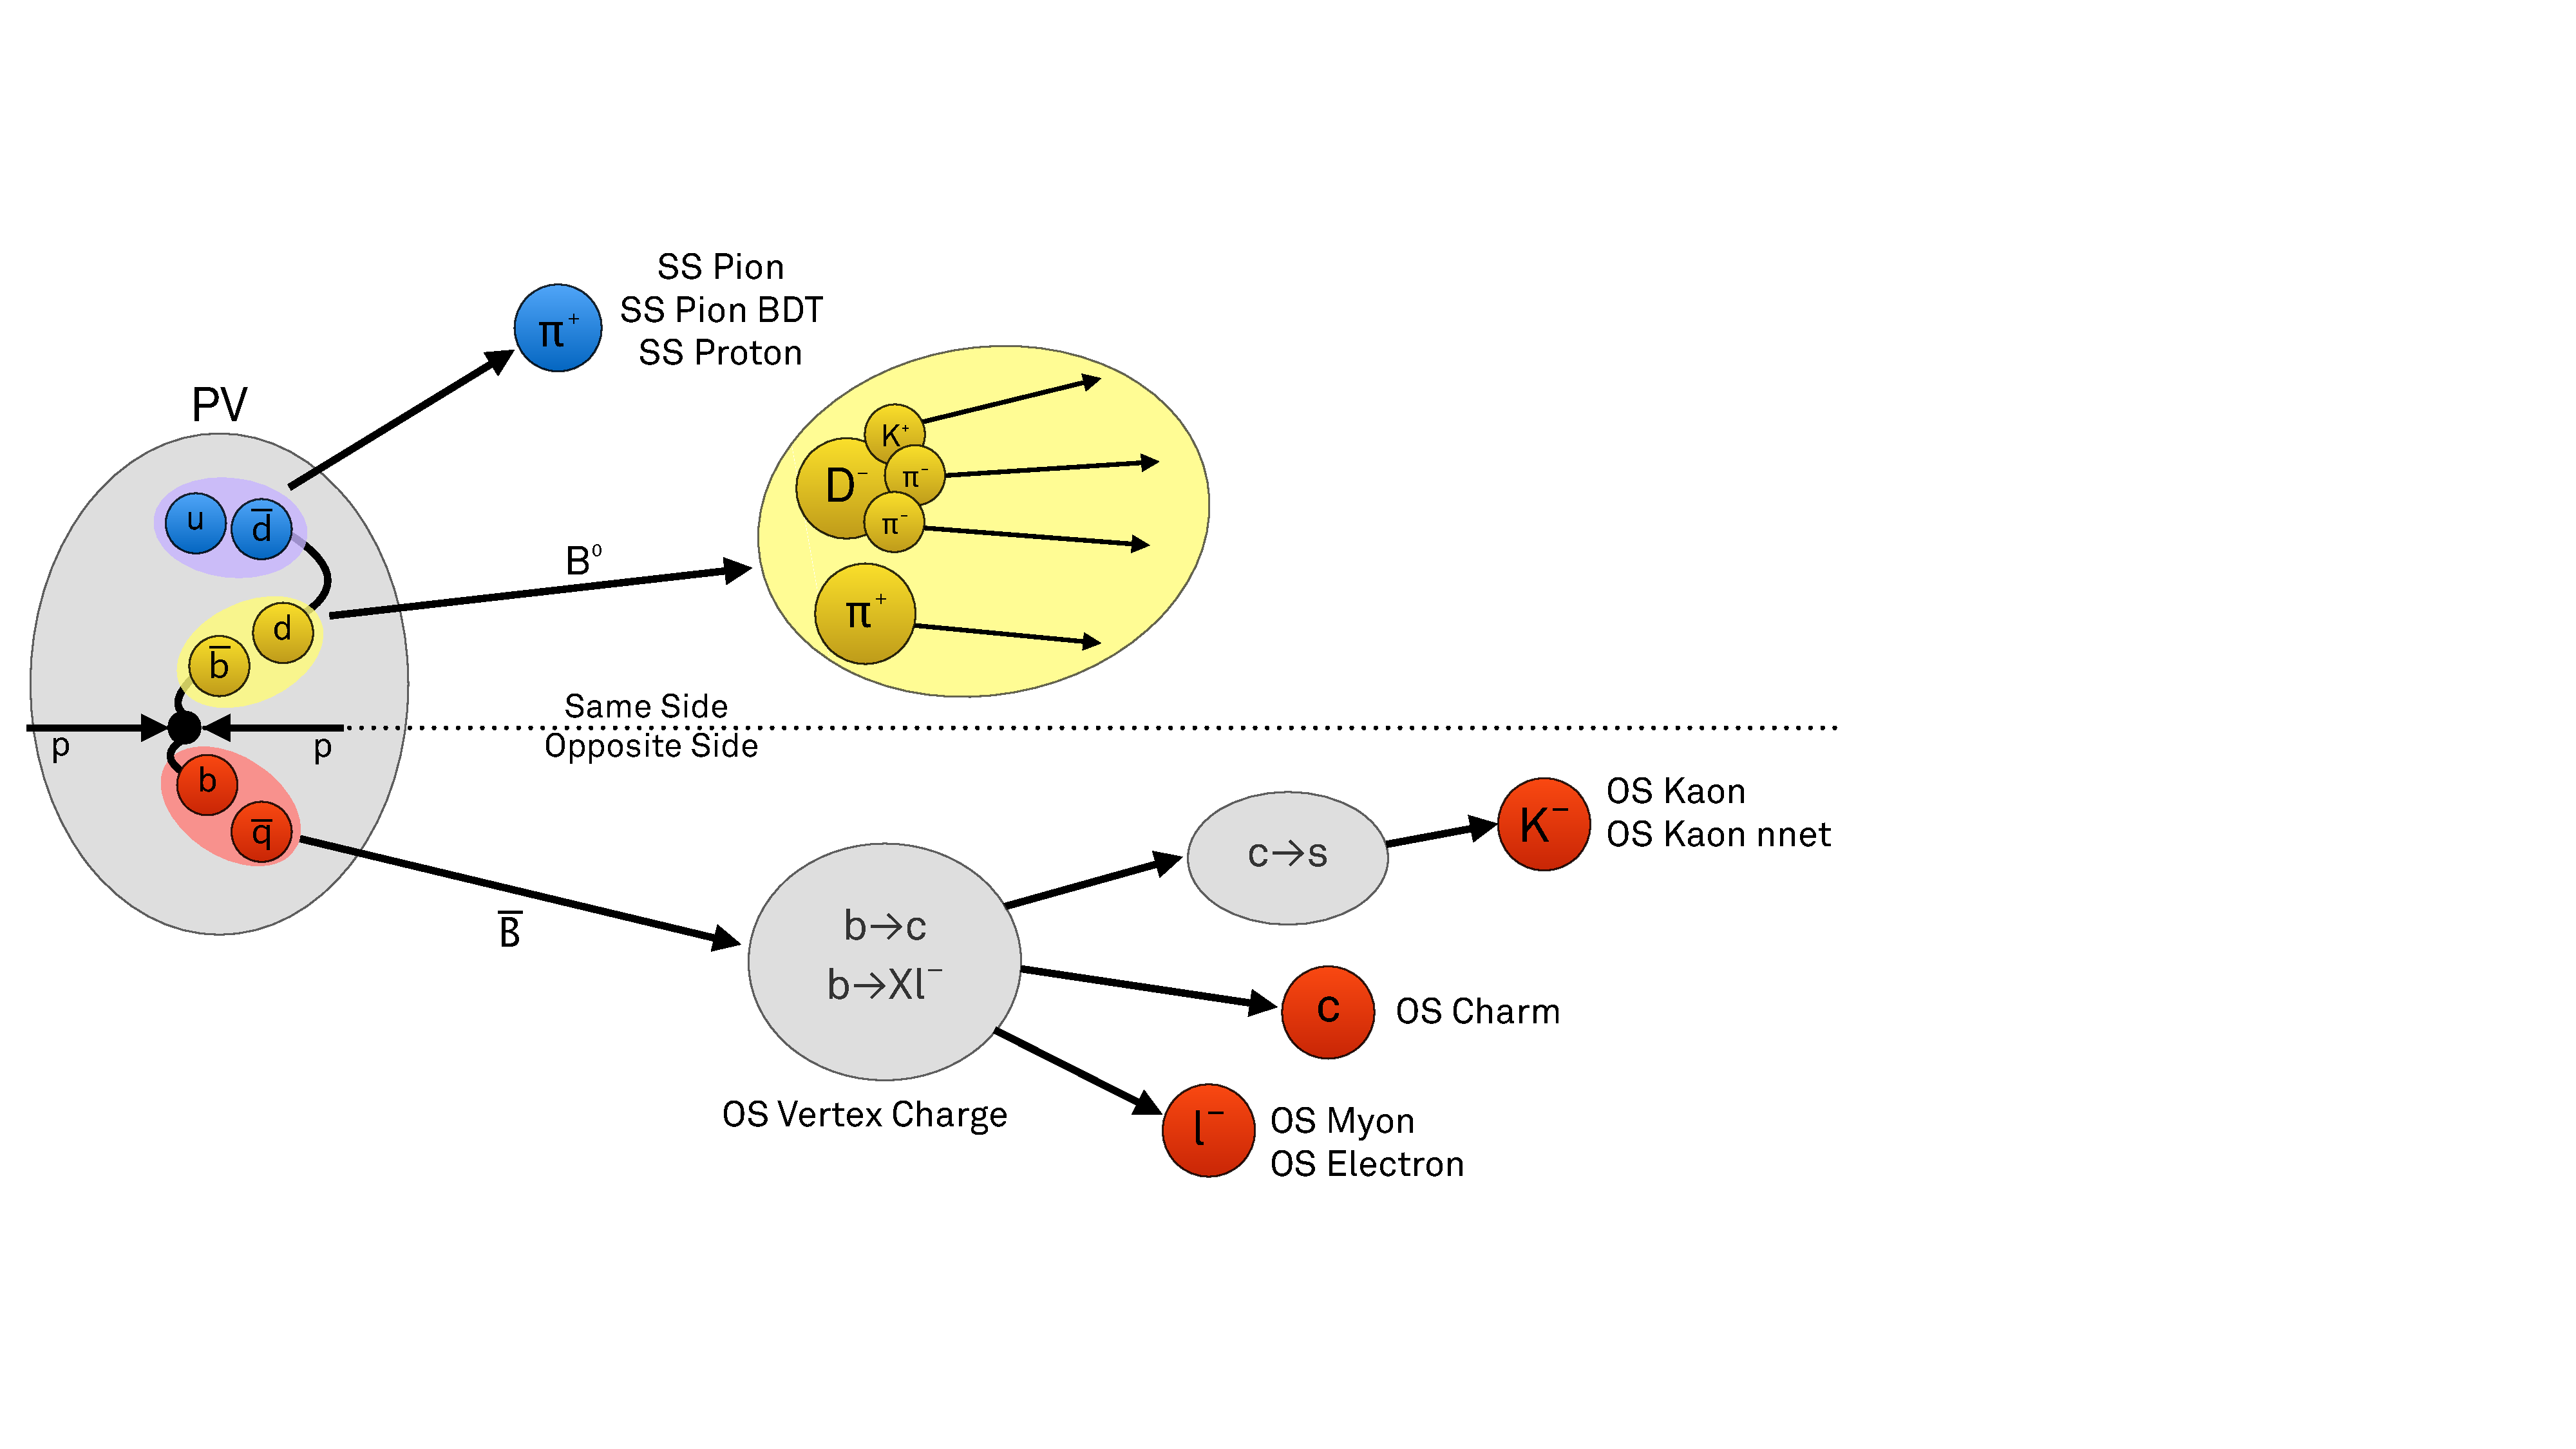
\includegraphics[width=\textwidth]{fig/FT_schema.pdf}
	\caption{Schematische Übersicht der Tagger, die in dieser Arbeit auf dem Kanal $\Bz\rightarrow D^-\pi^+$ kalibriert wurden.}
	\label{fig:flavourtagging} 
\end{figure}   

\section{Charakteristische Größen des Flavour Taggings}\label{sec:FTgrosse}

Jeder Tagger gibt zu jedem Kandidaten eine individuelle Entscheidung $d$ über den anfänglichen Flavour des \B-Mesons aus. Bei dieser Entscheidung, auch tag genannt, gibt es drei Möglichkeiten: als \Bz (\bquarkbar\dquark) getagged, als \Bzb (\bquark\dquarkbar) getagged oder ungetagged ($d=1$ entspricht einem \bquarkbar-Quark, $d=-1$ einem \bquark-Quark und $d=0$ einem ungetaggten Kandidaten). Außerdem erhält man zu jedem Kandidaten eine mistag-Wahrscheinlichkeit $\eta$, die eine Selbsteinschätzung der Wahrscheinlichkeit ist, mit der der Tagger bei einem Kandidaten falsch liegt. Da dies jedoch nur eine Abschätzung des Taggers über die Qualität seiner Entscheidung ist, wird die tatsächliche, kalibrierte Wahrscheinlichkeit mit der der Tagger falsch liegt mit 
\begin{equation}
\omega=\frac{N_{\text{R}}}{N_{\text{R}}+N_{\text{W}}}\label{eq:omega}
\end{equation}
dem true-mistag oder der true-mistag-Wahrscheinlichkeit bezeichnet. Dabei sind $N_{\text{R}}$ die Anzahl korrekt getaggter Ereignisse und $N_{\text{W}}$ die Anzahl falsch getaggter Ereignisse. Auf Monte-Carlo lässt sich nach Gleichung \eqref{eq:omega} aus den Truth-Informationen eine wahre true-mistag-Wahrscheinlichkeit berechnen, während auf Daten nur eine kalibrierte true-mistag-Wahrscheinlichkeit ermittelbar ist. Beachtet man diese Unsicherheit über den Anfangszustand nun für die gemessene Mischungsasymmetrie der \B-Mesonen (Gleichung \eqref{eq:mixing}) erhält man
\begin{equation}
\begin{split}
A_{\text{mix}}^{\text{tag}}&=\frac{\left(1-\omega\right)N_\text{unmixed}+\omega N_\text{mixed}-\left(1-\omega\right)N_\text{mixed}-\omega N_\text{unmixed}}{\left(1-\omega\right)N_\text{unmixed}+\omega N_\text{mixed}+\left(1-\omega\right)N_\text{mixed}+\omega N_\text{unmixed}}\\
&=\left(1-2\omega\right)\frac{N_\text{unmixed}-N_\text{mixed}}{N_\text{unmixed}+N_\text{mixed}}=\left(1-2\omega\right)\cos(\dm t).\label{eq:mischung}
\end{split}
\end{equation}
Analog dazu erhält man für eine gemessene \CP-Asymmetrie (Gleichung \eqref{eq:cpv})
\begin{equation}
A_\CP^{\text{tag}}=\left(1-2\omega\right)\frac{2\mathcal{Im}(\lambda_f)}{1+\left|\lambda_f\right|^2}\sin\left(\dm t\right).
\end{equation}
Man erkennt, dass durch die experimentelle Unsicherheit, die durch das Flavour Tagging hinzukommt, die Amplituden beider Asymmetrien um den gleichen Faktor abgeschwächt werden. Bei einer true-mistag-Wahrscheinlichkeit von $\omega=0{,}5$ würden so beide Asymmetrien im Experiment verschwinden. Dieser Faktor wird Dilution $D$ genannt: 
\begin{equation}
D=1-2\omega
\end{equation}
Die einzelnen Tagger unterscheiden sich weiterhin in ihren Effizienzen. So ist die Anzahl der gettagten Ereignisse nicht für alle Tagger gleich, sodass  man die Taggingeffizienz
\begin{equation}
\varepsilon=\frac{N_{\text{R}}+N_{\text{W}}}{N_{\text{R}}+N_{\text{W}}+N_{\text{U}}}
\end{equation}
definiert, bei der neben Kandidaten mit einem Tag ($N_\text{R}$ und $N_\text{W}$) auch ungetaggte Kandidaten ($N_\text{U}$) berücksichtigt werden. Weiterhin wird die effektive Taggingeffizienz
\begin{equation}
\varepsilon_\text{eff}=\varepsilon D^2
\end{equation}
eingeführt. Über diese lassen sich einzelne Tagger nun untereinander in ihrer Leistung vergleichen. So ist die effektive Taggingeffizienz $\varepsilon_\text{eff}$ auch ein Maß für die statistische Größe des zu untersuchenden Datensatzes. Multipliziert man die Anzahl Ereignisse eines Datensatzes mit dieser effektiven Taggingeffizienz $\varepsilon_\text{eff}$, so erhält man die Anzahl Kandidaten, die man bei einem perfekt getaggten Datensatz für die gleiche statistische Aussagekraft auf die Messung einer physikalischen Observablen wie \dmd oder $\sin\left(2\beta\right)$ benötigen würde. Dabei bedeutet perfekt getaggter Datensatz, das für jeden Kandidaten eine korrekte Tag-Entscheidung mit einem true-mistag von $\omega=0$ getroffen wurde.\\
Die bisher eingeführten Größen, speziell der true-mistag, beachtet keine Asymmetrie im Tagging zwischen \Bz- und \Bzb-Mesonen. Zieht man diese hinzu, lässt sich eine true-mistag $\omega$ für getaggte \Bz-Mesonen und $\overline{\omega}$ für getaggte \Bzb-Mesonen definieren. Der bisher verwendete true-mistag ist dann als mittlerer true-mistag 
\begin{equation}
\widetilde{\omega}=\frac{\omega+\overline{\omega}}{2}
\end{equation}
zu betrachten. Somit lässt sich eine mistag-Asymmetrie $\Delta\omega=\omega-\overline{\omega}$ definieren.

\section{Opposite Side Tagging}\label{sec:ostagging}

Beim Opposite Side Tagging wird der Hadronisierungsprozess des \bquark-Quarks ausgenutzt, welches nicht das \B-Meson des Signalzerfalls bildet. Dazu werden zum Einen einzelne Teilchen wie Elektronen, Myonen, Kaonen oder \D-Mesonen identifiziert, die im Zusammenhang mit Hadronisierungs- und Zerfallsprozessen dieses sogenannten Opposite Side \bquark-Quarks entstehen, zum Anderen nutzt einer der Tagger die Ladung von Spuren, die aus einem gemeinsamen Sekundärvertex kommen, der nicht mit dem Signal \B assoziiert ist (Abbildung \ref{fig:flavourtagging}). Da das Opposite Side \B-Meson unabhängig vom Signal \B-Meson sein sollte, also unabhängig von dessen Hadronisierungsprozess, können die Tagger sowohl für {{\ensuremath{\B^0_\dquark}}\xspace}-, als auch für  \Bs-Mesonen gleich verwendet werden. Im Folgenden soll nun in Anlehnung an \cite{tagging} auf die einzelnen Tagger eingegangen werden.
\begin{itemize}
\item Der OS Myon Tagger nutzt Myonen aus semileptonischen \B-Zerfällen um eine Tagentscheidung zu fällen. Davon ausgehend, dass das Opposite Side \B-Meson nicht gemischt hat, lässt sich aus der Ladung des Myons auf den anfänglichen Flavour des \B-Mesons schließen. Um tatsächlich Myonen der Opposite Side zu rekonstruieren, werden unterschiedliche Schnitte angewendet. Beiträge aus $\bquark\rightarrow\cquark\rightarrow\lepton$, was die falsche Ladung und damit den falschen Tag zur Folge hätte, werden beispielsweise durch einen Schnitt auf den Transversalimpuls $\pt>\SI{1{,}2}{GeV\per c}$ unterdrückt. Wenn nach den verschiedenen Selektionsschritten noch mehrere Myonenkandidaten übrig bleiben, wird das Myon mit dem höchsten Transversalimpuls $\pt$ für die Tagentscheidung genutzt.
\item Der OS Elektron Tagger funktioniert analog zum OS Myon Tagger. Auch hier gibt die Ladung eines Elektrons aus einem semileptonischen Zerfall des Opposite Side \B-Mesons Aufschluss über den anfänglichen Flavour des \B-Mesons. Die Elektronenselektion funktioniert ebenfalls durch einfache rechtwinklige Schnitte, wobei zusätzlich hilfreiche Variablen für die Elektronenidentifikation genutzt werden. Zu diesen gehört das Verhältnis der Teilchenenergie $E$, gemessen im \ecal und des Impulses $p$ des Elektronkandidaten. Dabei wird $E/p>0{,}8$ gefordert. Ebenfalls analog zum Myon-Tagger wird bei mehreren Elektronenkandidaten der Kandidat mit dem höchsten Transversalimpuls \pt für die Tagentscheidung gewählt
\item Der OS Kaon Tagger nutzt Kaonen aus der Zerfallskette $\bquark\rightarrow\cquark\rightarrow\squark$. Aus der Ladung des Kaons lässt sich wiederum auf den Flavour des \B-Mesons schließen, nimmt man an, dass das Opposite Side \B-Meson nicht gemischt hat. Bei dem schnittbasierten OS Kaon Tagger werden ebenfalls rechtwinklige Schnitte angewendet, um den Kaonkandidaten zu selektieren. Abschließend wird bei mehreren Kaonkandidaten wieder der Kandidat mit dem höchsten Transversalimpuls \pt gewählt. Beim Tagging mit OS-Kaonen gibt es zusätzlich eine Neuentwicklung, den OS Kaon nnet. Dieser selektiert die Kaonen nicht über rechtwinklige Schnitte, sondern nutzt ein neuronales Netz. So erhält man zwar deutlich mehr getaggte Ereignisse, die mistag-Wahrscheinlichkeiten sind jedoch im Mittel größer.
\item Der OS Vertex Charge Tagger ist der einzige Tagger, der keine Einzelteilchen rekonstruiert, sondern die gesamte gewichtete Ladung eines zum Opposite Side \B-Mesons assoziierten Sekundärvertex (SV) für seine Tagentscheidung nutzt. Dabei wird zunächst aus zwei Spuren ein Sekundärvertex rekonstruiert, wobei aus allen Spuren das Spurenpaar gewählt wird, das die höchste Wahrscheinlichkeit besitzt aus dem Opposite Side \B-Meson zu stammen. Anschließend werden nach einigen geometrischen und kinematischen Schnitten weitere Spuren zu dem gebildeten SV hinzugefügt. Aus diesen Spuren wird anschließend die gewichtete Ladung des SV
\begin{equation}
Q_\text{Vtx}=\frac{\sum_{i}\pt^k(i)Q_i}{\sum_{i}\pt^k(i)}
\end{equation}
gebildet. Der Parameter $k$ ist dabei dahingehend optimiert, eine maximale effektive Taggingeffizienz $\varepsilon_\text{eff}$ zu liefern.
\item Bei dem OS Charm Tagger handelt es sich ebenfalls um eine Neuentwicklung. Er trifft seine Entscheidungen basierend auf rekonstruierten \D-Mesonen, die vor allem aus der Zerfallskette $\bquark\rightarrow\cquark$ entstammen. Dabei gibt im Falle eines geladenen \D-Mesons dessen Ladung direkt Aufschluss über den anfänglichen Flavour des \B-Mesons, bei einem ungeladenen \D-Meson die Ladung des Kaons, in das das \D-Meson zerfällt. Die \D-Kandidaten werden dabei über einen Boosted Decision Tree (BDT) rekonstruiert. Der OS Charm Tagger wurde dabei, bei einem geringen Überlapp mit den anderen Taggern, auf eine maximale effektive Taggingeffizienz $\varepsilon D^2$ optimiert, sodass er im Vergleich zu den anderen Taggern relativ kleine Taggingeffizienzen $\varepsilon$ bei allerdings auch guten mistag-Vorhersagen liefert.
\end{itemize}
Die einzelnen Tagger können kombiniert werden, um die unterschiedlichen Vorhersagen zu nutzen und die effektive Taggingeffizienz $\varepsilon D^2$ des Datensatzes zu erhöhen. Dabei wird die kombinierte Wahrscheinlichkeit, dass das \B-Meson ein \bquark-Quark enthält, berechnet als
\begin{equation}
P(\bquark)=\frac{p(\bquark)}{p(\bquark)+p(\bquarkbar)} \hspace{1cm}\text{und}\hspace{1cm}P(\bquarkbar)=1-P(\bquark)
\end{equation}
wobei die Wahrscheinlichkeiten $p(\bquark)$ und $p(\bquarkbar)$ als
\begin{equation}
p(\bquark)=\prod_{i}\left(\frac{1+d_i}{2}-d_i\left(1-\eta_i\right)\right)
\end{equation}
und
\begin{equation}
p(\bquarkbar)=\prod_{i}\left(\frac{1-d_i}{2}+d_i\left(1-\eta_i\right)\right)
\end{equation}
definiert sind. Dabei sind $d_i$ die Entscheidungen und $\eta_i$ die mistag-Vorhersagen der einzelnen Tagger. Die kombinierte Entscheidung und mistag-Vorhersage ergibt sich für $P(\bquark)>P(\bquarkbar)$ nun zu $d=-1$ und $\eta=1-P(\bquark)$ und für $P(\bquark)<P(\bquarkbar)$ zu $d=1$ und $\eta=P(\bquark)$.\\
In der Flavour Tagging Software ist eine Kombination der OS Tagger direkt implementiert. Diese Standard OS Kombination enthält aktuell den OS Myon, den OS Elektron, den OS Kaon und den OS Vertex Charge Tagger, da es sich bei diesen um die bereits etablierten Tagger handelt.

\section{Same Side Tagging}

Beim Same Side Tagging werden direkt Abhängigkeiten bei der Hadronisierung des Signal \B-Mesons ausgenutzt. Im Falle eines \Bz (\bquarkbar\dquark) bleibt beispielsweise ein freies \dquarkbar-Quark, das zu einem Pion oder Proton hadronisieren kann. Im Falle eines \Bs (\bquarkbar\squark) bleibt ein freies \squarkbar-Quark, das zu einem Kaon hadronisieren kann. Für Pionen und Kaonen sind zwei beispielhafte Hadronisierungsprozesse in Abbildung \ref{fig:FThadronisierung} dargestellt.
\begin{figure}[htpb]
	\centering
		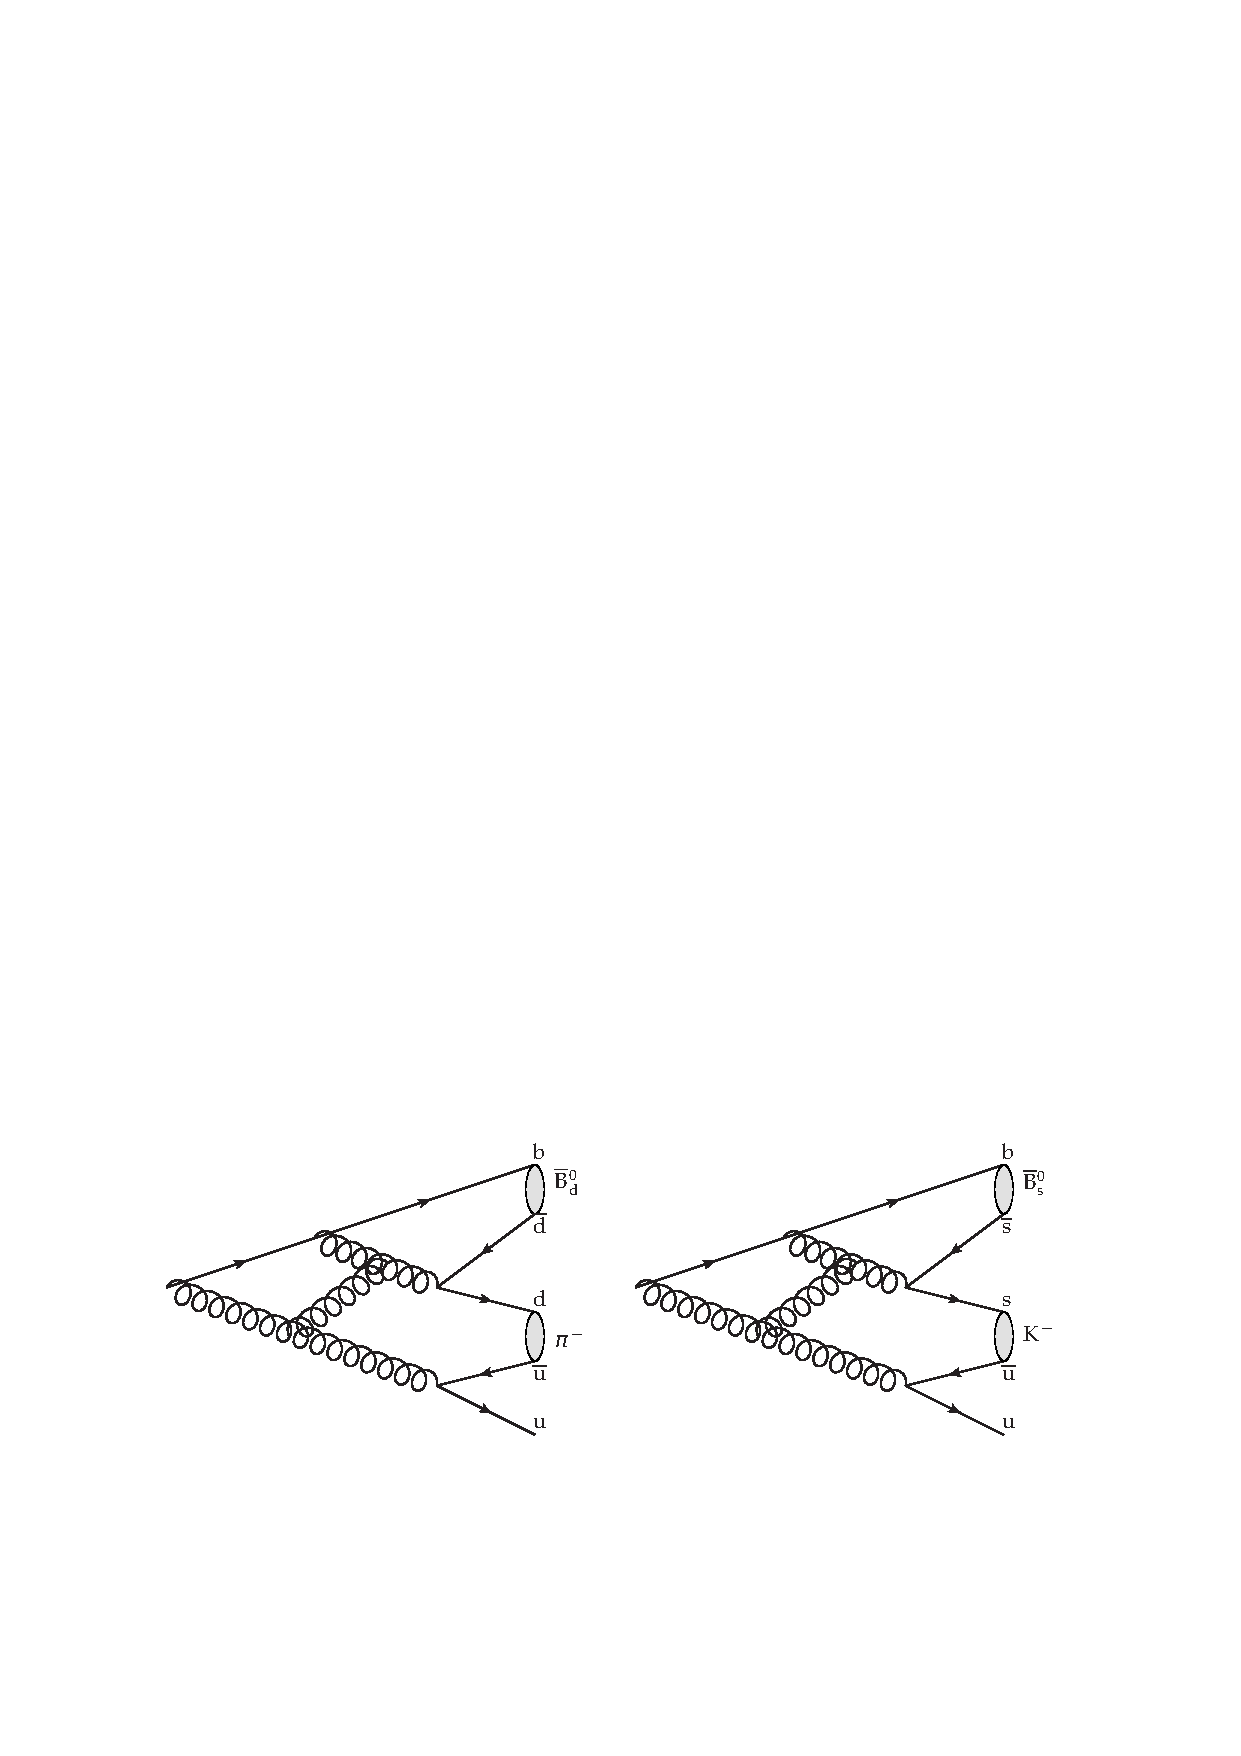
\includegraphics[width=0.8\textwidth]{fig/FThadronisierung.pdf}
	\caption{Feynmandiagramme der \Bz und \Bs Hadronisation. \cite{tagging}}
	\label{fig:FThadronisierung} 
\end{figure} 
Die einzelnen Tagger sollen nun im Folgenden wiederum in Anlehnung an \cite{tagging} genauer vorgestellt werden.
\begin{itemize}
\item Der SS Pion Tagger nutzt in \Bz-Zerfällen die Ladung eines im Hadronisationsprozess entstehenden Pions. Dabei werden sowohl Pionen, die direkt aus einem zusätzlichen \dquark-Quark (Abbildung \ref{fig:FThadronisierung} links) beim \Bz stammen genutzt, als auch Pionen aus höher angeregten \B-Zuständen, wie dem {{\ensuremath{\B^{0*}}}\xspace} oder dem {{\ensuremath{\B^{0**}}}\xspace}. Die Selektion des SS Pion Taggers basiert, ebenso wie bei den meisten OS Taggern, auf rechtwinkligen Schnitten. Dabei werden ähnliche Kriterien wie bei der Auswahl für die OS Tagger angewendet, um geeignete Pionen zu rekonstruieren, wie Schnitte auf den Transversalimpuls der Kandidaten. Ebenso wird, falls mehrere Pion Kandidaten vorliegen, analog der Kandidat mit dem höchsten Transversalimpuls \pt  für die Tagentscheidung gewählt. Ähnlich wie bei dem OS Kaon Tagger gibt es auch bei dem SS Pion Tagger eine Neuentwicklung, die auf einer multivariaten Methode basiert. Der SS Pion BDT Tagger nutzt zur Selektion  eines geeigneten Pion Kandidaten einen BDT. Auch hier erhält man mit der multivariaten Methode deutlich mehr getaggte \B-Mesonen, allerdings im Schnitt auch schlechtere mistag-Vorhersagen.
\item Der SS Proton Tagger ist ebenso wie der SS Pion BDT eine Neuentwicklung. Er funktioniert, wie die beiden SS Pion Tagger, für \Bz-Mesonen Zerfälle. Die Teilchenselektion basiert auf einem BDT und hat hohe Anzahlen an getaggten Ereignissen ($\varepsilon>\SI{30}{\%}$) und im Schnitt eher hohe mistag-Vorhersagen ($\langle\eta\rangle>0{,}4$).
\item Der SS Kaon Tagger ist für \Bs-Meson-Zerfälle entwickelt worden und arbeitet für diese analog zum SS Pion Tagger für \Bz-Ereignisse. Da in dieser Arbeit das Flavour Tagging im Kanal $\Bz\rightarrow\Dm\pip$ untersucht werden soll, wird auf den SS Kaon Tagger an dieser Stelle nicht weiter eingegangen.
\end{itemize}
Neben der möglichen Verwendung des SS Pion, des SS Pion BDT und des SS Proton Tagger für \Bz-Ereignisse lassen sich alle drei natürlich auch für \Bu-Ereignisse (\bquarkbar\uquark) nutzen um das Flavour Tagging zu kalibrieren. 

\section{Vorgehen bei der Tagging Kalibrierung}

Wie in Abschnitt \ref{sec:FTgrosse} bereits erwähnt, liefert jeder Tagger für jedes Ereignis eine Abschätzung $\eta$ der mistag-Wahrscheinlichkeit. Diese Abschätzung muss für die Analyse von \CP-Asymmetrien auf die true-mistag-Wahrscheinlichkeiten $\omega$ kalibriert werden. Dabei geht man von einem linearen Zusammenhang der Form
\begin{equation}
\widetilde{\omega}(\eta)=p_0+p_1\cdot\left(\eta-\langle\eta\rangle\right)\label{eq:linear}
\end{equation}
aus. Dabei ist $\langle\eta\rangle$ der Mittelwert aller $\eta$-Werte eines Taggers. Durch Subtrahieren dieses Wertes von den einzelnen $\eta$-Werten werden die Parameter $p_0$ und $p_1$ dekorreliert. Bei einem perfekt kalibrierten Tagger gilt, dass $p_0=\langle\eta\rangle$ und $p_1=1$ entspricht. Analog dazu lässt sich die mistag-Asymmetrie parametrisieren:
\begin{equation}
\Delta\omega(\eta)=\Delta p_0+\Delta p_1\cdot\left(\eta-\langle\eta\rangle\right)\label{eq:lineardelta}
\end{equation}
Die verschiedenen Tagger werden nun auf unterschiedlichen Zerfallskanälen kalibriert, sodass ein Satz aus Werten für die Parameter für $p_0$, $p_1$, $\Delta p_0$ und $\Delta p_1$ inklusive statistischer und systematischer Unsicherheiten entsteht. Für die globale Kalibrierung wird dann ein bestimmter Kanal verwendet, und die Abweichungen in den weiteren geprüften Kanälen werden genutzt um systematische Unsicherheiten zu ermitteln. Der Kanal \BdToDpi wurde zuletzt nicht verwendet, soll nun aber wieder in die Kombination der Flavour Tagging Gruppe eingehen.\\
Die möglichen Verfahren zur Tagging Kalibrierung unterscheiden sich für die Zerfälle von ungeladenen \B-Mesonen auf Monte-Carlo und Daten grundsätzlich und werden in den nächsten beiden Abschnitten erläutert.   

\subsection{Daten}\label{sec:kalibrierungDaten}

Da auf Daten der wahre Flavour für ungeladene \B-Mesonen nicht bekannt ist, lässt sich dieser nicht nach Gleichung \eqref{eq:omega} durch einfaches Abzählen bestimmen. Allerdings bietet die Mischungsasymmetrie (Gleichung \eqref{eq:mischung}) eine Möglichkeit $\omega$ zu bestimmen.\\ 
Im Folgenden wird dazu der Datensatz in Kategorien der mistag-Vorhersage $\eta$ eines Taggers geteilt. Dann werden Masse und Zerfallszeit simultan in diesen Kategorien der mistag-Vorhersage $\eta$ gefittet. Der Massenfit geschieht dabei, um besser zwischen den Signal und Untergrund-Komponenten zu unterscheiden. Bei der Parametrisierung der Zeit sind die Gleichungen \eqref{eq:uebergang1}, \eqref{eq:uebergang2}, \eqref{eq:uebergang3} und \eqref{eq:uebergang4} an die Unsicherheiten des Flavour Taggings anzupassen. Dabei wird hier weiter der Spezialfall der \Bz-Mesonen mit $\Gamma_H\approx\Gamma_L$ und $\left|\tfrac{q}{p}\right|=1$ betrachtet:
\begin{equation}
\begin{split}
\Gamma^\text{exp}\left(\Bzb\to f\right)&=\left(1-\overline{\omega}\right)\Gamma\left(\Bzb\to f\right)+\omega\cdot\Gamma\left(\Bz\to f\right)\\
\Gamma^\text{exp}\left(\Bz\to f\right)&=\left(1-\omega\right)\Gamma\left(\Bz\to f\right)+\overline{\omega}\cdot\Gamma\left(\Bzb\to f\right)\\
\Gamma^\text{exp}\left(\Bzb\to\overline{f}\right)&=\left(1-\overline{\omega}\right)\Gamma\left(\Bzb\to\overline{f}\right)+\omega\cdot\Gamma\left(\Bz\to\overline{f}\right)\\
\Gamma^\text{exp}\left(\Bz\to\overline{f}\right)&=\left(1-\omega\right)\Gamma\left(\Bz\to\overline{f}\right)+\overline{\omega}\cdot\Gamma\left(\Bzb\to\overline{f}\right).
\end{split}
\end{equation}
Mithilfe der Tagentscheidung $d$ und dem Mischungszustand $\xi$, der zwischen gemischten und ungemischten \B-Mesonen unterscheidet, lassen sich die vier unterschiedlichen Fälle zu
\begin{equation}
\Gamma^\text{exp}\left(\hat{B}\to\hat{f}\right)=\frac{1}{2}e^{-\Gamma t}\left[\left(1-d\Delta\omega\right)+\xi\left(1-2\widetilde{\omega}\right)\cos\left(\dmd t\right)\right]
\end{equation}
zusammenfassen, wobei mögliche asymmetrische mistag-Wahrscheinlichkeiten $\omega$ und $\overline{\omega}$ mit einem mittleren true-mistag $\widetilde{\omega}$ und der mistag-Asymmetrie $\Delta\omega$ beschrieben werden. Mit einer Unterscheidung zwischen den vor dem Zerfall gemischten und ungemischten Zuständen ist der Fit hier also sensitiv auf die true-mistag-Wahrscheinlichkeit $\widetilde{\omega}$ in jeder Kategorie. Nach der Bestimmung von mittleren mistag-Vorhersagen $\eta$ in jeder Kategorie lassen sich so erhaltene $(\eta,\widetilde{\omega})$-Paare nun mit ein linearer Zusammenhang nach Gleichung \eqref{eq:linear} beschreiben. Da der Fit mit der tag-Entscheidung $d$ ebenso auf die mistag-Asymmetrie $\Delta \omega$ sensitiv ist, lässt sich diese analog gegen die Kategoriemittelwerte der mistag-Vorhersage $\eta$ auftragen und nach Gleichung \eqref{eq:lineardelta} kalibrieren.\\
Neben dieser in der Flavour Tagging Arbeitsgruppe zumeist durchgeführten Methode Tagger zu kalibrieren, soll außerdem ein weiteres Verfahren vorgestellt werden. Dabei werden die mistag-Wahrscheinlichkeiten $\eta$ in Wahrscheinlichkeiten $P_\text{tag}(\bquarkbar)$, dass das betroffene Teilchen ein \bquarkbar-Quark enthält, umgerechnet. Bei einer Tagentscheidung $d=-1$ ergibt sich also $P_\text{tag}(\bquarkbar)=\eta$ und bei einer Tagentscheidung $d=1$ erhält man $P_\text{tag}(\bquarkbar)=1-\eta$. Für ungetaggte Teilchen ist $P_\text{tag}(\bquarkbar)=0{,}5$. Nun wird der Datensatz in Kategorien dieser Wahrscheinlichkeit $P_\text{tag}(\bquarkbar)$ eingeteilt und der Zusammenhang zur wahre Wahrscheinlichkeit $P_\text{true}(\bquarkbar)$ kalibriert. Nun lassen sich die Bereiche für \bquarkbar ($0{,}5<P_\text{tag}(\bquarkbar)<1$) und für \bquark ($0<P_\text{tag}(\bquarkbar)<0{,}5$) einzeln mit linearen Funktionen der Form
\begin{equation}
P_\text{true}(P_\text{tag})=p_0+p_1\cdot\left(P_\text{tag}-\langle P_\text{tag}\rangle\right)\label{eq:linearPB},
\end{equation}
kalibrieren, wobei die Parameter in diesem Kontext für \Bz-Mesonen (\bquarkbar\dquark) im Weiteren mit $p_0$ und $p_1$ und für \Bzb-Mesonen (\bquark\dquarkbar) mit $\overline{p_0}$ und $\overline{p_1}$ bezeichnet werden sollen. Die Zentralwert für \Bz- und \Bzb-Mesonen werden dann mit $\widetilde{p_0}$ und $\widetilde{p_1}$ beschrieben.\\
Hintergrund dieser Methodik ist, dass die verschiedenen Tagger intern mit der Wahrscheinlichkeit $P(\bquarkbar)$ rechnen.

\subsection{Monte-Carlo}\label{sec:mckalibrierung}

Auf Monte-Carlo ist der generierte (wahre) Produktionsflavour der \B-Mesonen bekannt. So lässt sich durch Vergleich zwischen dem bekannten initialen Flavour eines Ereignisses und der entsprechenden Entscheidung eines Taggers erkennen, ob der Tagger mit seiner Entscheidung richtig oder falsch lag. Unterteilt man den Datensatz nun in Bins der mistag-Vorhersage $\eta$ des Taggers, kann man in jedem Bin den mittleren wahren true-mistag $\omega$ nach Gleichung \eqref{eq:omega} berechnen. Durch Berechnen der Mittelwerte der $\eta_i$ in jedem Bin lassen sich die zugehörigen mittleren mistag-Vorhersagen der Tagger berechnen. Trägt man nun die $\omega$ in Abhängigkeit von $\eta$ auf lässt sich der lineare Zusammenhang aus Gleichung \eqref{eq:linear} bestimmen. Dabei sind die $\eta$-Werte nun die Mittelwerte der $\eta_i$ und $\omega$ die wahren true-mistag-Wahrscheinlichkeiten in den einzelnen Bins.\\
Neben dieser einfachen Methode ließe sich auf Monte-Carlo auch ein simultaner Fit umsetzen um eine Kalibrierung durchzuführen. Da auf Monte-Carlo jedoch der Untergrund explizit ausgeschaltet werden kann, wird hier neben dem Lebenszeitfit zur Bestimmung der mistag-Wahrscheinlichkeiten $\widetilde{\omega}$  und mistag-Asymmetrien $\Delta\omega$ kein zusätzlicher Massenfit benötigt.

